\chapter{Metodología, Diseño, Software o Implementación propuesta}\label{Cap_02}
\lettrine[lines=2,nindent=0pt]{S}{}e debe explicar la metodología, diseño, software o implementación propuesta, donde se detalle lo siguiente:

\begin{itemize}
\item El problema que resolverá
\item Descripción general de la solución propuesta
\item Descripción detallada de cada fase, etapa, módulo, etc.
\item En esta sección se describe tu aportación de la tesis, por lo que es necesario conjuntar todo el conocimiento previo del marco teórico, estado del arte y metodologías estudiadas para que tu trabajo sea fundamentado, sustentado y factible de desarrollar o implementar.
\item Debe tener calidad argumentativa, es decir, que sea congruente con lo investigado hasta ahora, marco teórico y estado del arte.
item referencia a la figura (figure \ref{fig:figure})
\item Tabla \ref{table:1} es un ejemplo de un elemento en \LaTeX{}.

\end{itemize}

\begin{figure}[H]
    \begin{center}
    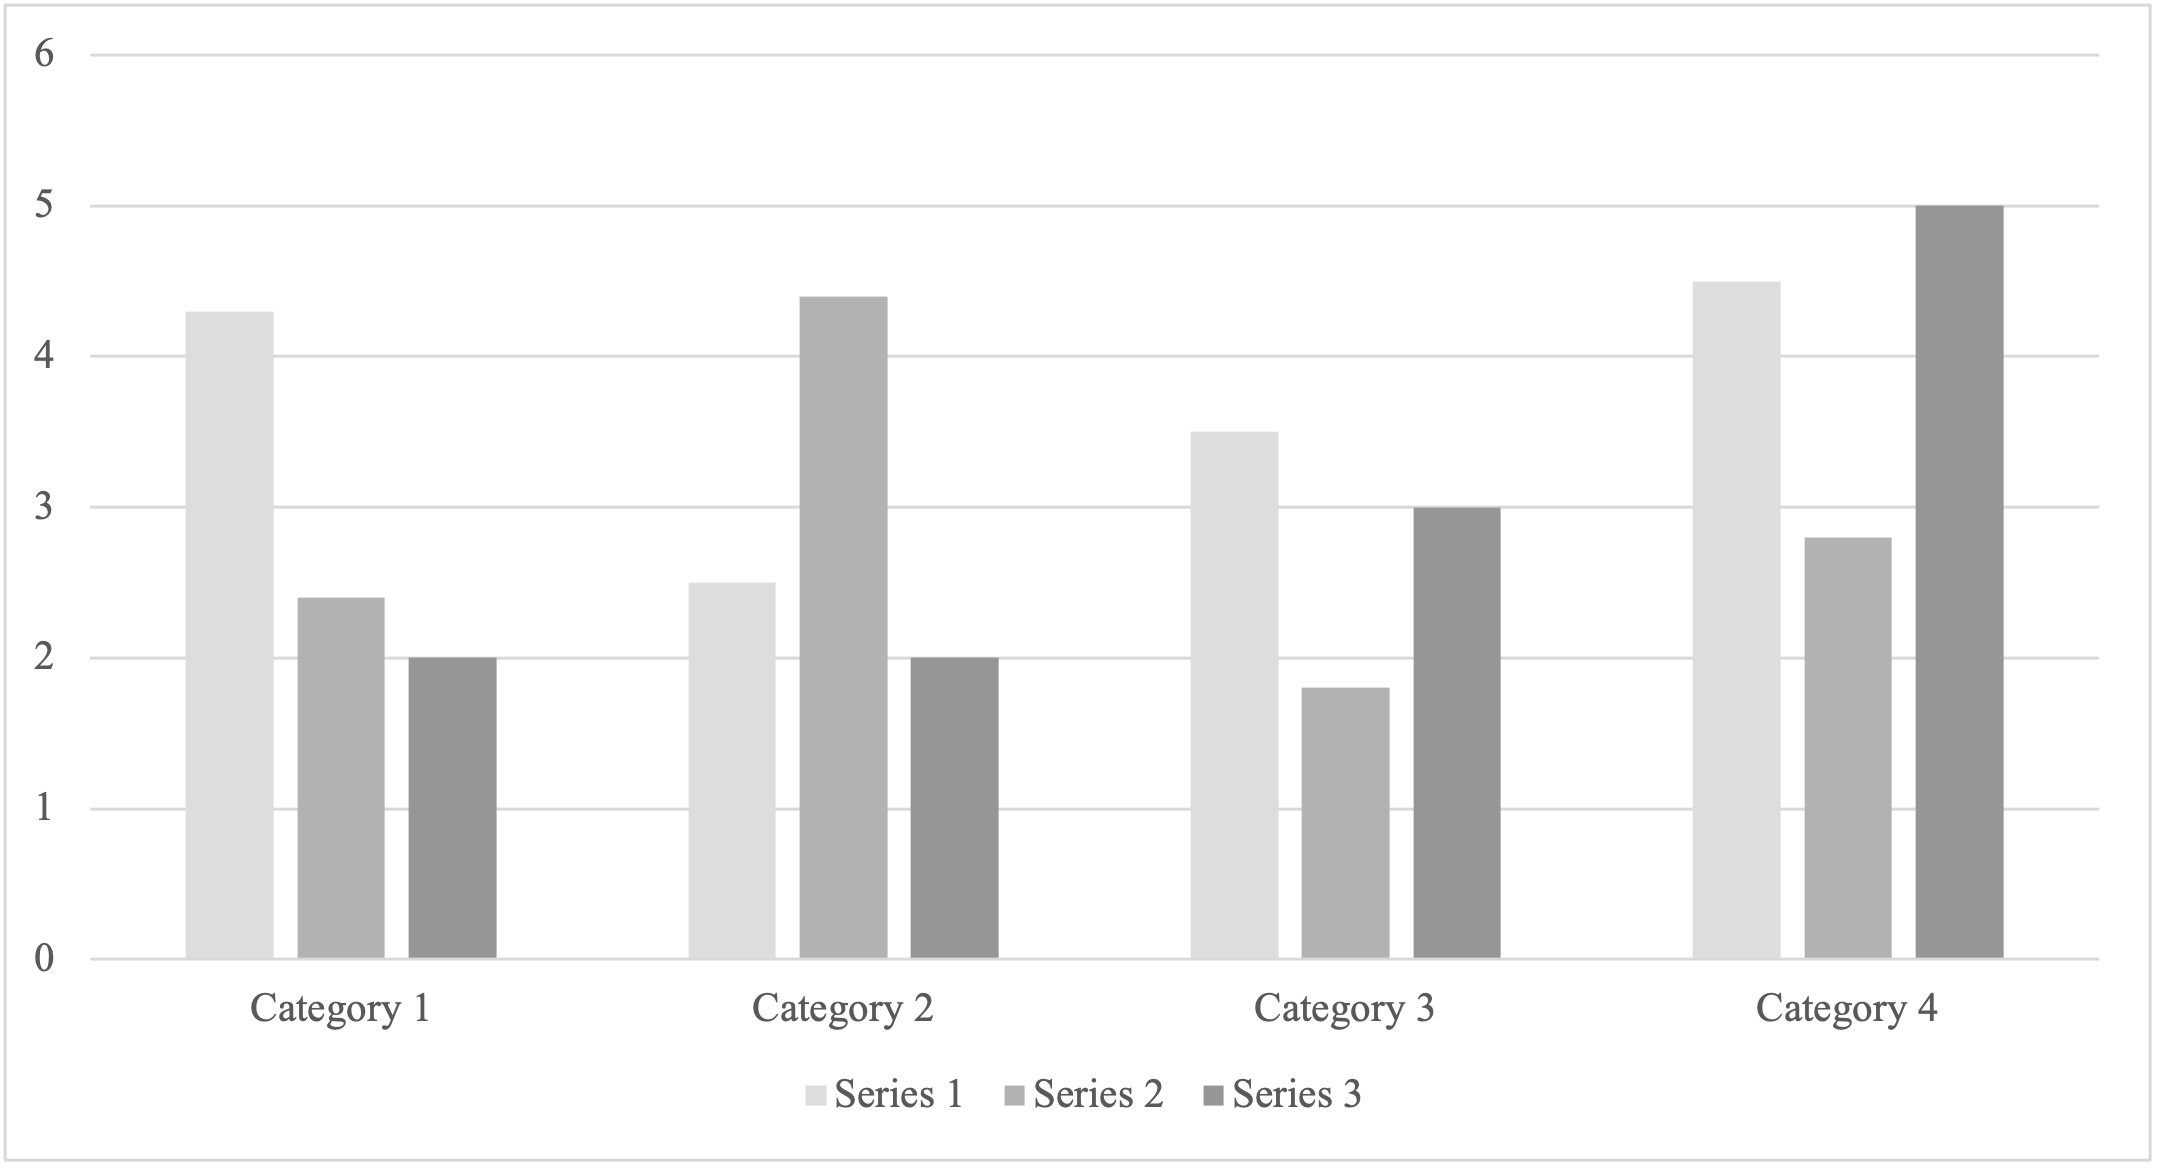
\includegraphics[width=.8\textwidth]{Cap_02/grafica.png}\caption[Metodología CRISP-DM]{Include all figures in their own section, following references (and footnotes and tables, if applicable).  Include a numbered caption for each figure.  Use the Table/Figure style for easy spacing between figure and caption.]}\label{fig:figure}
    \end{center}
    \end{figure}



    \begin{table}[h!]
    \centering
    \caption{Table to test captions and labels.}
    \label{table:1}
    \begin{tabular}{c c c c} 
     \hline
     Col1 & Col2 & Col2 & Col3 \\ [0.5ex] 
     \hline
     1 & 6 & 87837 & 787 \\ 
     2 & 7 & 78 & 5415 \\
     3 & 545 & 778 & 7507 \\
     4 & 545 & 18744 & 7560 \\
     5 & 88 & 788 & 6344 \\ [1ex] 
     \hline
    \end{tabular}
    \end{table}